\documentclass[12pt, a4paper, oneside]{book}%, oneside to be removed if printing needed

\usepackage[headings]{fullpage}
\usepackage{setspace}
\usepackage{soul}
% \usepackage[top=1.5cm,right=1.5cm,bottom=1.5cm,left=1.5cm]{geometry}
% \usepackage{fancyhdr}
% \setlength{\headheight}{20pt} 
% \usepackage{graphics}
\usepackage{graphicx}
\usepackage{float}
\usepackage{subfig}
\usepackage{array}
% \usepackage{xtab}
\usepackage{multirow}
\usepackage{booktabs}
\usepackage{appendix}
\usepackage[pdfborder={0 0 0}, colorlinks=true, linkcolor=black, citecolor=blue]{hyperref}
\usepackage[printonlyused]{acronym}
\usepackage{algorithmic}
\usepackage{algorithm}
\usepackage{ifpdf}
\usepackage{listings}
%\usepackage{epstopdf}%added
% \setlength{\parindent}{0pt}

%\graphicspath%added

\newcommand{\submissionDay}{XX}
\newcommand{\submissionMonth}{July}
\newcommand{\submissionYear}{2015}
\newcommand{\submissionDate}{\submissionDay~\submissionMonth,~\submissionYear}
\newcommand{\typeOfThesis}{Bachelor Thesis}

\newcommand{\titleOfThesisOne}{Mission impossible: Disproving failed conjectures}

\newcommand{\authorOfThesis}{Heba Aamer Anwar Mohamed}
\newcommand{\supervisorOne}{Professor Dr. Stephan Schulz}
%\newcommand{\supervisorTwo}{Sup 2}
%\newcommand{\supervisorThree}{Sup 3}

\newcommand{\includefig}[4]{
    \begin{figure}[ht]
     \centering
      \includegraphics[width=#1\textwidth]{images/#2}
      \caption{#3}
      \label{#4}
    \end{figure}
}

\newcommand{\includefigWSC}[5]{
    \begin{figure}[ht]
     \centering
      \includegraphics[width=#1\textwidth]{images/#2}
      \caption[#3]{#4}
      \label{#5}
    \end{figure}
}

\newcommand{\includeeps}[4]{
\includefig{#1}{#2.eps}{#3}{#4}
}

\newcommand{\includeepsWSC}[5]{
\includefigWSC{#1}{#2.eps}{#3}{#4}{#5}
}


\ifpdf
\pdfinfo {
	/Author (\authorOfThesis)
	/Title (\titleOfThesisOne)
	/Subject (\typeOfThesis)
	/Keywords ()
	/CreationDate (D:20090707085533)
}
\fi

\begin{document}
% \overfullrule=5pt
\pagestyle{plain}
\pagenumbering{Roman}

\newcommand{\titlePage}{

\thispagestyle{empty}
\begin{center}
	\textbf{Department of Computer Science}\\[1mm]
	\textbf{Duale Hochschule Baden-W\"urttemberg Stuttgart}\\[1mm]
	
\includegraphics[scale=0.53]{pictures/Logo_DHBW_Stuttgart_4c.jpg}
	
	\vspace{2cm}
	\doublespacing
	{\Huge \textbf{\titleOfThesisOne}}\\
	\singlespacing
	\vspace{2cm}
	{\large \textbf{\typeOfThesis}}\\
	
	\vfill
	\parbox{1cm}{
  		\begin{large}
    			\begin{tabbing}
       			Author: \hspace{2cm}  
        			\=\authorOfThesis\\[2mm]
      			Supervisor: 
        			\>\supervisorOne\\[2mm]
			%	\>\supervisorTwo\\[2mm]
			%	\>\supervisorThree\\[2mm]
      			Submission Date: 
        			\>\submissionDate\\
    			\end{tabbing}
  		\end{large}
	}\\
\end{center}
\clearpage
}
%++++++++++++++++++++++++++++++++++++++++++++++++++++++++++++++++++++
\titlePage
%\thispagestyle{empty}\ \clearpage
%\titlePage
%++++++++++++++++++++++++++++++++++++++++++++++++++++++++++++++++++++
\thispagestyle{empty}
This is to certify that:
\begin{itemize}
\item[(i)] the thesis comprises only my original work toward the Bachelor Degree
\item[(ii)] due acknowledgement has been made in the text to all other material used
\end{itemize}

\vspace{2cm}
\begin{flushright}
\rule[0mm]{6cm}{0.2mm}\\
\authorOfThesis\\
\submissionDay~\submissionMonth,~\submissionYear\\
\end{flushright}
\clearpage


\chapter*{Acknowledgements}
\addcontentsline{toc}{chapter}{Acknowledgements}
\label{chap:ack}


\paragraph{}
First of all, I have to thank my supervisor Professor Dr. Stephan Schulz for his continuous support and understanding through out the last six months and for setting an example for real researcher to me.

\paragraph{}
Many thanks for Prof. Peter Baumgartner and Dr. Renate Schmidt for their help in understanding their paper, and answering my very long questions.

\paragraph{}
I thank my Egyptian professors and doctors for their help when being abroad specially Associate Prof. Haythem Ismail, and Dr. Hany El-Sharkawy. 

\paragraph{}
I really can not express how much love I have for my whole family, specially my grandma, father, mother and brother, for their support and encouraging to achieve this stage of my education. Without them in my life, it would have been very hard to have any successes. Your existence in my life is priceless.

\paragraph{}
And last but not least, My friends the ones who travelled with me and the others who were in Egypt. You were a gift from God to me. Thank you for your help, and encouraging. 


\chapter*{Abstract}
% \addcontentsline{toc}{chapter}{Abstract}
\label{chap:abstract}

In the past few decades the field of automated theorem proving (ATP) has been flourishing and improving a lot by the enormous amount of research devoted to it. That interest came from its importance as well as its various uses in different fields such as mathematical reasoning.



ATP comes along with another process which is model generation/computation/construction from a certain (counter) satisfiable specification/problem. Model generation has usages that ATP alone wont have the effect that it has with it, and that could be noticed in Software/Hardware verification, debugging various systems.



Here in this project we added a model generation technique for a subclass in First Order Logic named Effectively Propositional Calculus in an existing theorem prover "E" where we transform the axioms of the specification into a certain form called range restricted form, and then after reaching saturation, we apply Bachmair and Ganzinger model construction technique to get the model.



Automated theorem proving has applications in mathematics, verification, common-sense reasoning, and many other domains. It can demonstrate the compliance of a system with certain requirements. However, it is often just as important to show that a desired property is not met. This can be done by constructing a counter-model, or, in simpler words, a counter-example. In this talk we describe the implementation of techniques that enable the theorem prover E to find such counter-examples for effectively propositional proof problems, and to give an explicit counter-models to the user.


\paragraph{}
\textbf{Keywords:} Automated Theorem Proving, Model Construction, Effectively propositional logic, Range Restricting Transformations, Theorem Prover E, Bachmair and Ganzinger Model Construction Technique.  
\tableofcontents
% \addcontentsline{toc}{chapter}{Contents}
\clearpage 

\pagestyle{headings}
\pagenumbering{arabic}

% \setlength\parskip{15pt}
\setlength\parskip{.5\baselineskip plus .2\baselineskip
	minus .4\baselineskip}
% \setlength\parskip{.5\baselineskip \@plus .1\baselineskip \@minus ..1\baselineskip}


\chapter{Introduction}\label{chap:intro}

	\nocite{*} 
	%TODO :: add this in better position	
	
	\paragraph{    Constructing Models} has a huge importance in many fields specially in debugging tasks. It helps in modelling and highlighting the existence of bugs. And because of this it is used extensively in the field of Software and Hardware verification, also in analyzing and verifying Theorems.

	\paragraph{    So a concrete example} to show its importance is the verification of Timsort, which was explained in details here \cite{TIMSORT}. Timsort is a hybrid sorting algorithm that was developed in 2002. It combines merge sort and insertion sort. And it was developed in the beginning to be used in python, but later on it was added to java. And today in Open JDK, Sun's JDK, and Android SDK it is the default sorting algorithm since it showed a great performance on real data. That resulted in using it in billions of devices because of the popularity of those platforms. In 2015, a formal verification for Timsort was tried to be done by a team using KeY, a verification tool for java programs that could be found here \url{http://www.key-project.org/}. And their analysis showed that the TimSort algorithm was broken and they found a bug and they corrected it, then after that they were able to formally verify the correction of the algorithm. And all the happened by the help of KeY. So it really beneficial to have models.

	\paragraph{    Having that importance in mind,} we needed in this project to have an explicit model given to user when running problems on the theorem prover E, specifically for a sub-class of \ac{fol} named \ac{epr}. And in order to achieve that goal, Transformations have been applied to the problem specification to transform it to a certain form, namely range restricted form. Afterwards, Bachmair and Ganzinger Model Construction Technique is applied to extract the explicit model from the saturated set of the problem specification. 


	\paragraph{    So a discussion of the work done} will be given in the following order. We will have a background on the topic in chapter \ref{chap:background}. Then in chapter \ref{chap:meth_and_impl} we will discuss the methodology followed and the implementation. Afterwards in chapter \ref{chap:test_and_val} we will explain the procedures followed to test the accuracy and efficiency of the implemented techniques. Moreover, A discussion of the results and related works will be found in chapter \ref{chap:res_and_lit}. Then a conclusion will be given in chapter \ref{chap:concl}. And last but not least a discussion for related future work will be in chapter \ref{chap:todo} 

\chapter{Background}\label{chap:background}


This chapter is devoted for introducing and familiarizing the reader to the theoretical concepts behind this project, and give the reader a background on the theorem prover E as well. So it will include the following sections:
	\begin{itemize}
		\item A background on \acf{fol} in section \ref{sec:c2s1} %TODO add a reference
		\item A background on \acf{epr} in section \ref{sec:c2s2} %TODO add a reference
		\item A background on Problem set in section \ref{sec:c2s3} %TODO add a reference
		\item A background on E in section \ref{sec:c2s4} %TODO add a reference
	\end{itemize}


\section{Background on first order logic topics} \label{sec:c2s1}

\ac{fol}, which is also known as first order predicate logic, is an expressive logic that allows us to formulate most of our spoken language sentences in a defined way such that it could be further handled with rules such as simplification, inference rules, etc.\\*
We could represent formulas in \ac{fol} in so many forms. So \ref{sub:c2s1s1} will be devoted to that part of background.\newline
Moreover, in general the universe of \ac{fol} is infinite because of the existence of the quantifiers and function terms. So in \ref{sub:c2s1s2} some topics related to that property will be mentioned including Herbrand Universe.\newline    
Also this project is concerned to a specific class of \ac{fol} its calculus named \ac{epr}, and this will be discussed in \ref{sub:c2s1s4}.

\subsection{Different forms of \ac{fol}}\label{sub:c2s1s1}
\ac{fol} can be represented in different forms. Even some algorithms need to work with specific one.
Moreover, there are some procedures that could transform a formula from one form to another.
Here in this part, we will discuss the most important forms and the relevant ones to the project.
\newline
1- general form\newline 
2- clausal normal form\newline
3- prenex normal form\newline
4- skolem normal form

\subsubsection{General Form}
General form

\subsubsection{Clausal normal form}
\ac{cnf}

\subsubsection{Prenex normal form}
\ac{pnf}

\subsubsection{Skolem normal form}
\ac{snf}

\subsection{The universe of \ac{fol}}\label{sub:c2s1s2}
Discuss the infinity of the universe in general.\newline
And then mention the Herbrand Universe. 

\subsection{Skolemization}\label{sub:c2s1s3}
Skolemization is the step that transforms \ac{pnf} formulas into \ac{snf}.
In which all the existentially quantified variables are removed and replaced by some function terms and its arguments are all the universally quantified variables appeared before the one in concern.\\
Example for a formula in \ac{pnf}:\newline
\begin{displaymath}
\exists W \forall X \forall Y \exists Z  \left(P(a,W,X,Y,Z)\right).  
\end{displaymath}\newline
After it transformed into \ac{snf}:\newline
\begin{displaymath}
\forall X \forall Y  \left(P(a,b,X,Y,f(X,Y))\right).  
\end{displaymath}

%TODO add link to the algorithm of the transformation in the appendix. 

\subsection{What is \ac{epr}}\label{sub:c2s2s1}
\acf{epr} or sometimes known as Bernays-Sch\"onfinkel class is a fragment of \acf{fol} in which all of its formulas follow the following format:

\begin{lstlisting}[caption=Format of \ac{epr} formula,label={lst:epr_format},breaklines=true,mathescape,frame=single]
                          $\exists *$ $\forall *$ $F$
  where $F$ is the formula.
  Moreover, $F$ has no proper functions symbols (all functions present are nullary ones "constants").
\end{lstlisting}

\ac{epr} fragment has a huge number of applications, e.g. Planning and Verifcation. 


\subsection{Example on \ac{epr}}\label{sub:c2s2s2}
Example for a formula in \ac{epr}:

\begin{lstlisting}[caption=Example for an \ac{epr} formula,breaklines=true,escapeinside={(*}{*)},frame=single]
(* \begin{displaymath}
		\exists X \exists Y \forall Z  \left(P(a,X,Y,Z)\right).
	\end{displaymath} *)
\end{lstlisting}


Keeping \ref{lst:epr_format} in mind, this will make every skolemized formula that originally was in \ac{epr} format have no proper function symbols. After transforming the above equation, it will be:

\begin{lstlisting}[caption=Example for a skolemized \ac{epr} formula,breaklines=true,escapeinside={(*}{*)},frame=single]
(* \begin{displaymath}
	\forall Z \left( P(a,b,c,Z) \right).
	\end{displaymath} *)
\end{lstlisting}



\subsection{Decidability and Universe of \ac{epr}}\label{sub:c2s2s3}
Since the domain of \ac{epr} formulas contains only constants, and the number of constants in a formula is finite. So Herbrand universe of \ac{epr} formulas is finite. From that we could prove that \ac{epr} fragment is a decidable fragment in \ac{fol}, because of the finite number of ground interpretations it can have.


\subsection{Equality in \ac{epr}}\label{sub:c2s2s4}
As we have mentioned before that \ac{epr} formulas will never contain proper function symbols. So terms will be one of two options:
\begin{itemize}
	\item constant
	\item variable
\end{itemize}


And since Equality may be added to \ac{fol} as discussed in subsection \ref{sub:c2s2s3}, then we should consider the case if the formulas are from the \ac{epr} fragment. Equations are in the following form $t1$ $\approx$ $t2$, where t1 and t2 are terms. And since terms in \ac{epr} are only variables and constants. So the ground case of the Equation will contain only of constants. This result is important and we will refer to it later in chapter \ref{chap:meth_and_impl}.
 



   



\section{Problem Set}\label{sec:c2s3}

\paragraph{}
TPTP problems are first order problems, that are considered benchmarks to measure the performance of the different automated theorem provers. A description for TPTP could be found in \cite{TPTP09}, and the problem set could be downloaded from \url{http://www.cs.miami.edu/~tptp/}. TPTP problem set consists of different categories of problems, or divisions in other words, such as : PUZ, NLP, and GRP. Those categories came from the scientific meaning of the different problems, e.g., NLP represents natural language processing problems.

\paragraph{}
TPTP has its own language; TPTP for problems and TSTP for solutions. TPTP language could be written in two formats. The first of them is FOF, which is first order form. While the second form is CNF, which is clause normal form. Having a unified language for problems and solutions had a great impact on the field of \ac{atp}. And this allows the integration of different \ac{atp} systems ,i.e., Automated theorem provers, since they have a specific language that could communicate in.  

\paragraph{}
The theorem prover iProver is clear example on the integration between the different automated theorem provers . According to \cite{korovin2013inst}, iProver does not do the step of clausification by itself. It uses other theorem provers to have this step done. It uses Vampire for having the problem in CNF format, and it can use E as well to do so. 

\paragraph{}
An example for a problem, i.e., GRP004-1 problem, from the TPTP problem set is given below in CNF format:

	\begin{minipage}{\textwidth}
	\begin{lstlisting}[caption=GRP004-1.p problem,basicstyle=\footnotesize,breaklines=true,frame=single]
%--------------------------------------------------------------------------
% File     : GRP004-1 : TPTP v6.1.0. Released v1.0.0.
% Domain   : Group Theory
% Problem  : Left inverse and identity => Right inverse exists
% Version  : [Cha70] axioms : Incomplete.
% English  : In a group with left inverses and left identity every element
%            has a right inverse.

% Refs     : [Luc68] Luckham (1968), Some Tree-paring Strategies for Theore
%          : [Cha70] Chang (1970), The Unit Proof and the Input Proof in Th
%          : [CL73]  Chang & Lee (1973), Symbolic Logic and Mechanical Theo
% Source   : [Cha70]
% Names    : Example 3 [Luc68]
%          : Example 4 [Cha70]
%          : Example 4 [CL73]
%          : EX4 [SPRFN]

% Status   : Unsatisfiable
% Rating   : 0.00 v5.4.0, 0.11 v5.3.0, 0.10 v5.2.0, 0.00 v2.1.0, 0.00 v2.0.0
% Syntax   : Number of clauses     :    5 (   0 non-Horn;   3 unit;   3 RR)
%            Number of atoms       :   11 (   0 equality)
%            Maximal clause size   :    4 (   2 average)
%            Number of predicates  :    1 (   0 propositional; 3-3 arity)
%            Number of functors    :    3 (   2 constant; 0-1 arity)
%            Number of variables   :   15 (   1 singleton)
%            Maximal term depth    :    2 (   1 average)
% SPC      : CNF_UNS_RFO_NEQ_HRN

% Comments : [Luc68] is actually the right to left version.
%--------------------------------------------------------------------------
cnf(left_inverse,axiom,
    ( product(inverse(X),X,identity) )).
cnf(left_identity,axiom,
    ( product(identity,X,X) )).
cnf(associativity1,axiom,
    ( ~ product(X,Y,U)
    | ~ product(Y,Z,V)
    | ~ product(U,Z,W)
    | product(X,V,W) )).
cnf(associativity2,axiom,
    ( ~ product(X,Y,U)
    | ~ product(Y,Z,V)
    | ~ product(X,V,W)
    | product(U,Z,W) )).
cnf(prove_there_is_a_right_inverse,negated_conjecture,
    ( ~ product(a,X,identity) )).
%--------------------------------------------------------------------------
	\end{lstlisting}
	\end{minipage}



\section{The theorem prover E} \label{sec:c2s3}
\subsection{What is E}
E is a fully automatic theorem prover for \ac{fol} with equality implemented in ANSI-C that was released in 1998. Moreover, It is a saturation-based theorem prover. The Calculus implemented in E is variant of the superposition calculus proposed in \cite{BAGA94}.


\subsection{What can E do}
Since superposition calculus is a refutation one. So the current state of E, that it could prove the un-satisfiability of set of axioms with the negation of the conjecture(s) by finding the empty clause, or returning the saturated set if the empty clause was not found and no more new clauses can be inferenced/simplified. 


The returned saturated set is considered a model in the sense that it satisfies all the formulae in the give specification. However, an explicit model for the specification is not provided. Worth mentioning that it is not guaranteed in E to terminate/halt for \ac{epr} problems. This could be seen from the performance of E in \ac{epr} problems as it does not terminate in more than 50\% of them. 



\subsection{The Code flow of E}
This part is devoted from giving a brief on the main procedure in E. Figure ~\ref{fig:e_code_flow} is a simplified version of the code flow in E.

	\begin{figure}[H]
		\centering
		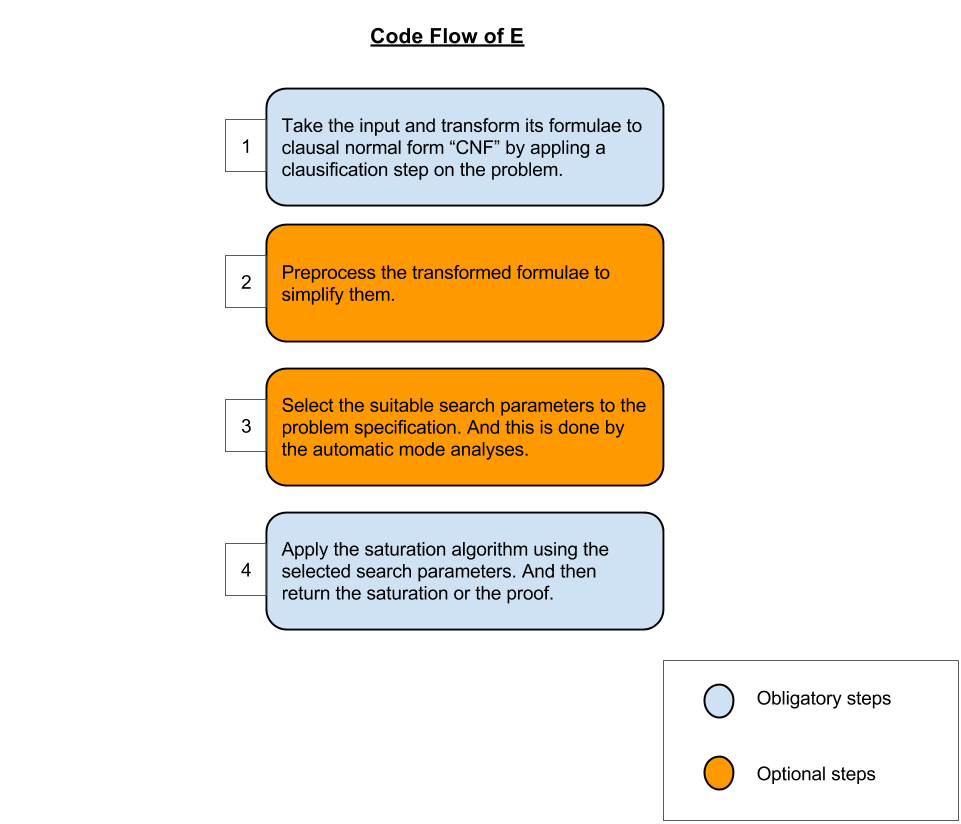
\includegraphics[scale=0.45]{pictures/e_code_flow.png}
		\caption{E Simplified code flow}\label{fig:e_code_flow}
	\end{figure}



\subsection{Latest results}
The latest results showed performance approaching 70\% over all the CNF and FOF problems of the TPTP problem set and this is according to \cite{E13}.
	

\chapter{Methodology and Implementation}\label{chap:meth_and_impl}

Methodology and Implementation

\section{Transformations}\label{sec:c3s1}
The methods applied in the project to extract the models follows the transformations discussed in \cite{BMUG06}. A brief on the original transformations will be given in \ref{sub:c3s1s1}.


Moreover, as mentioned before that this project is concerned with a sub-class of \ac{fol} which is \ac{epr} some simplifications to the transformations were made as the removed steps will have no meaning in the context of \ac{epr} problems. Those simplifications will be discussed in \ref{sub:c3s1s2}.

	\subsection{Original transformations}\label{sub:c3s1s1}
	\paragraph{The original procedures} discussed in \cite{BMUG06} generally work for all sub-classes of \ac{fol}. Those procedures should be applied to a given set of axioms in a specific form called implication form, sometimes it is called a sequent as in here ---ref---, which is explained here -- , and here -- to know how to transform to that form. Moreover, those transformations are guranteed to terminate for any given problem set, which is a gain for us since some of the \ac{epr} problems were not terminating in the original configurations of E.  
%TODO :: to add a reference later

	\subsubsection{What are the Transformations}
	
		\paragraph{} 
		\textbf{The Transformations} are series of procedures, mainly about changing the clauses to certain form named range restricted form. Since the transformations deal with clauses in implication form, then we could define \textbf{Clauses in range restricted form} \ul{to be clauses in which all the variables that appear in the succeedent must exist in the anticedent as well}.
	
		\paragraph{} 
		\textbf{An example for a range restricted clause} is found below:
			\begin{lstlisting}[caption=Range Restricted Clause Example,frame=single,mathescape]			
		
		$ \forall X \forall Y  \left( P(X) \wedge Q(Y) \longrightarrow R(X, Y) \right). $				
		
	where the $\textbf{antecedent}$ here is $ P(X) \wedge Q(Y) $;
	whereas the $\textbf{succeedent}$ is $ R(X, Y) $.
 			\end{lstlisting}
		
		
		\paragraph{} 
		\textbf{For a reason} why this range restricted form will help would be ??
%TODO :: add the reason later

	 \subsubsection{How do the transformations work}
	 
		\paragraph{} 
		\textbf{Transformations} add a domain predicate to the specification that will help in finding the Model by saying what are the elements of the domain, or the elements of the universe in other words.\par
		Moreover, There are three types of procedures in the transformations:	
		\begin{itemize}
			\item \textbf{Range restricting transformations}
			 \hfill \\ are the first two transformations, and they are the most important type of them. All the rest were added to enhance and improve the range restricting ones. They are responsible for transforming the input clauses to the range restricted form and enumerating the universe/domain of the problem in a way or another. Only one of the two transformations should applied, since they perform the same functionality but in different ways. The two transformations are:
			 	\begin{itemize}
			 		\item \ac{crr}: it enumerates the Herbrand Universe in a naive simple way. 
			 		\item \ac{rr}: it was introduced to improve the naive implementation of the \ac{crr}. So it only adds elements to the domain only when it is needed.
			 	\end{itemize}
			
			\item \textbf{Shifting transformations}
			 \hfill \\ are the second two transformations. They are optional to be used. They complement one another not replace each other. They were introduced mainly to prevent the non-termination of the transformations and to prevent generating and redundant and unpleasant clauses from the steps in \ac{rr} as well. And the two shifting transformations are:
			 	\begin{itemize}
			 		\item \ac{bs}
			 		\item \ac{pf}
			 	\end{itemize}
			
			\item \textbf{\ac{bl}}
			 \hfill \\ is the last transformation and it is optional as well. And It was introduced to detect periodicity that may occur because of function terms. 
		\end{itemize}
		
		\paragraph{} \textbf{Their order of application} is:
			\begin{enumerate}
				\item One of the two range restricting \ac{crr} or \ac{rr}
				\item The Partial Flattening \ac{pf}
				\item The Basic Shifting \ac{bs}
				\item The Blocking \ac{bl} 
			\end{enumerate}			 
		Where the output of a lower number transformation is the input to the higher one. A Flow Chart that summarizes what was explained will be found in Figure ~\ref{fig:original_transformations_flow}.
		
		\begin{figure}[H]
			\centering
 		 	\scalebox{0.38}
 			{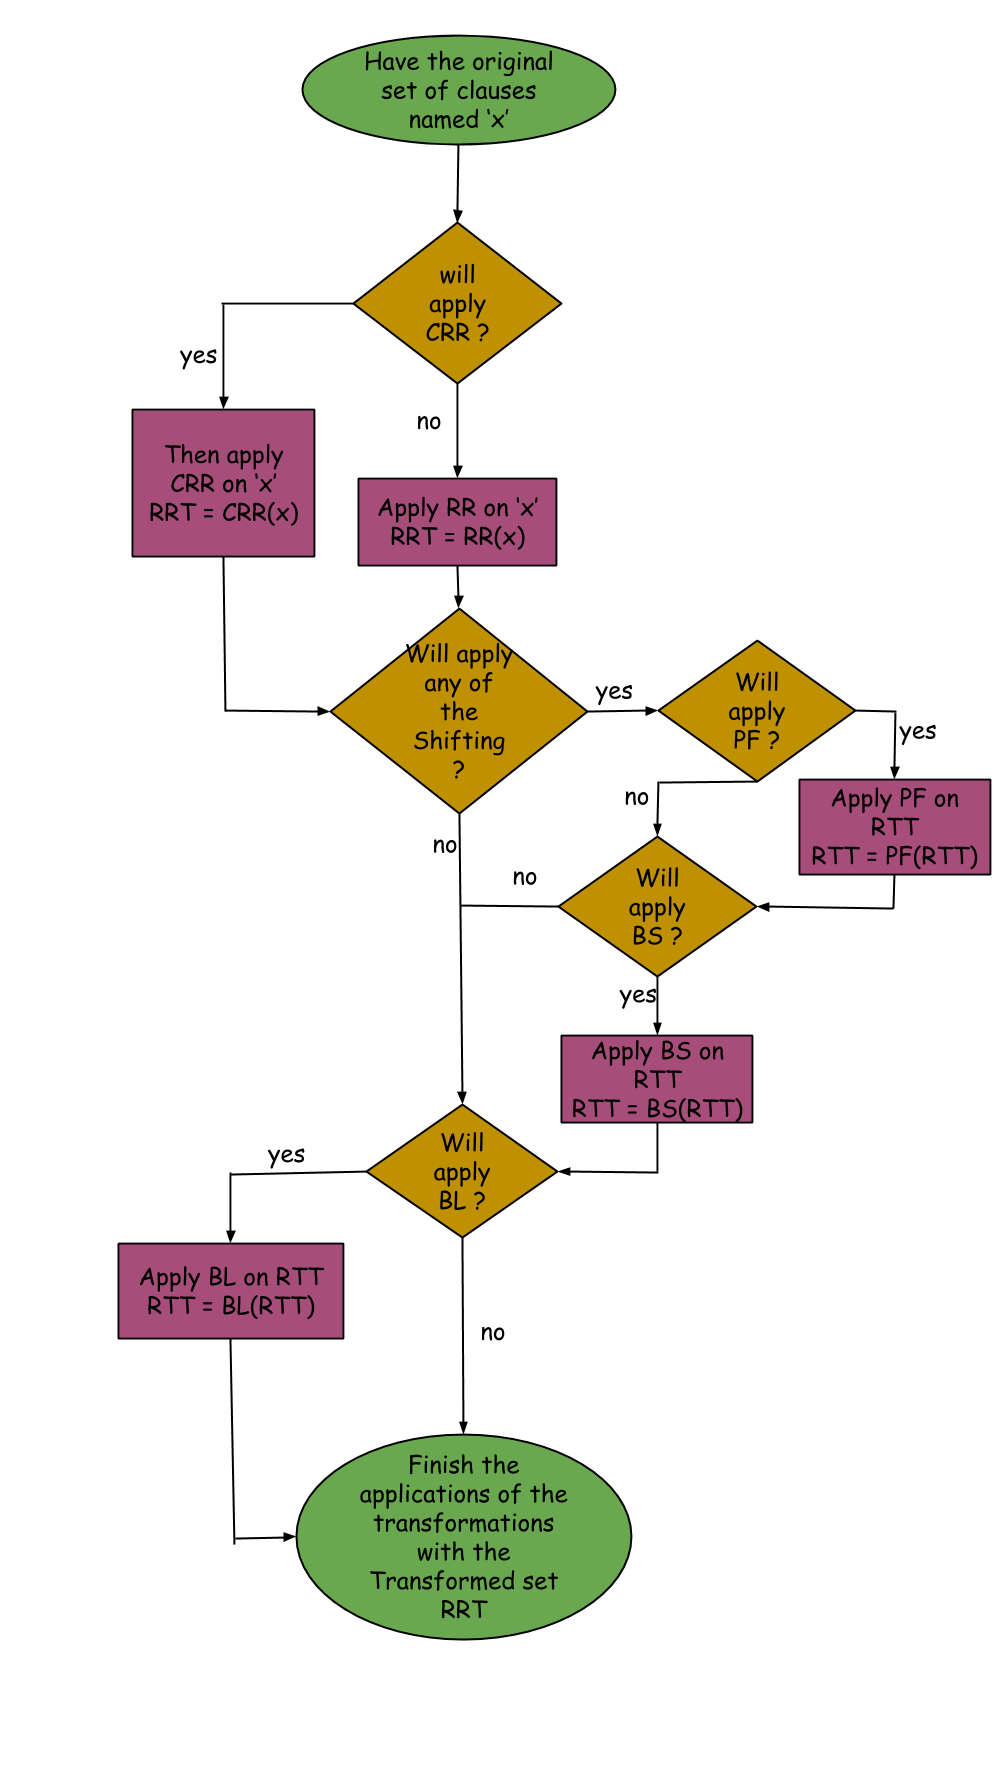
\includegraphics{pictures/Original_transformations_flow.png}}
 			\caption{Flow of the original transformations}\label{fig:original_transformations_flow}
		\end{figure}
	\subsection{Simplified transformations}\label{sub:c3s1s2}

This part is concerned about discussing the simplifications that were added to the original transformations highlighted in \ref{sub:c3s1s1}.
\\
Keeping in mind the definition of \ac{epr} as mentioned here in \ref{sub:c2s1s4}.
\\
So the following were made to each of the procedures:
\\
1- Every step that only deals with proper function symbols is removed since they are not existing in \ac{epr}.
\\
2- Any step or procedure that was introduced because of the existence of problems because of proper function symbols were removed as well. Ex.: pf, sh, and bl.
\\
\\
Therefore the resultant simplified procedures are the following:
\\
For crr:
\\
(0) Initialization. Initially, let crr(M) := M.
\\
(1) Add a constant. Let dom be a “fresh” unary predicate symbol not in ΣP , and let c
be some constant. Extend crr(M) by the clause dom(c) ← . (The constant c can
be “fresh” or belong to Σ f .)
\\
(2) Range-restriction. For each clause H ← B in crr(M), let {x1 , . . . , xk } be the set of
variables occurring in H but not in B . Replace H ← B by the clause
H ← B ∧ dom(x1 ) ∧ · · · ∧ dom(xk ).
\\
\\
For rr:
\\
(0) Initialization. Initially, let rr(M) := M.
\\
(1) Add a constant. Same as Step (1) in the definition of crr.
\\
(2) Domain elements from clause bodies. For each clause H ← B in M and each atom
P(t1 , . . . ,tn ) from B , let P(s1 , . . . , sn ) be the term abstraction of P(t1 , . . . ,tn ) and let α be the corresponding abstraction substitution. Extend rr(M) by the set
{dom(xi )α ← P(s1 , . . . , sn ) | 1 ≤ i ≤ n and xi → ti ∈ α}.
\\
(3) Range-restriction. Same as Step (2) in the definition of crr.
\\
(4) Domain elements from ΣP . For each n-ary P in Σ p , extend rr(M) by the set
{dom(xi ) ← P(x1 , . . . , xn ) | i ≤ i ≤ n}.


  
	

\section{Code Flow}
\chapter{Testing and Validation}\label{chap:test_and_val}
Testing and Validation


%\section{Section Name} \label{sec:s1}
%Some sample text with an \ac{ac}, some citation \cite{citeKey1}, and some more \ac{ac2}.


%\section{Another Section}
%Reference to Section \ref{sec:s1}, and reuse of \ac{ac} nad \ac{ac2} with also full use of %\acf{ac2}.

\section{Efficiency}
\subsection{Memory Efficiency}
The first part of the implementation which is related to applying the transformations to the the clause set introduces no memory leaks to the whole program.
%TODO add number of problems checked upon
\\
Tools to check this: \\
1- Script implemented in E for giving a summary on the allocated and de-allocated memory structures, and the results showed that they are equal.
\\
Ex.:\\
\# -------------------------------------------------
\\
\# Total SizeMalloc()ed memory: 68536168 Bytes (131507 requests)
\\
\# Total SizeFree()ed   memory: 68536168 Bytes (131507 requests)
\\
\# New requests:    214 (   197 by SecureMalloc(),     17 by SecureRealloc())
\\
\# Total SecureMalloc()ed memory: 277647 Bytes
\\
\# Returned:       214 (   214 by FREE(),              0 by SecureRealloc())
\\
\# SecureRealloc(ptr):     19 (    17 Allocs,      0 Frees,      2 Reallocs)
\\
\# -------------------------------------------------
\\
\\
2- Tool named 'valgrind' which also showed the same results as the above script.

\section{Accuracy of the transformations}
The results of ./edisprover part is the same as the author of the paper implemented program in all the tested problems.
\chapter{Results and Literature review}\label{chap:res_and_lit}
Results and Literature review

\chapter{Conclusion}\label{chap:concl}

Conclusion

\chapter{Future Work}\label{chap:todo}
	\paragraph{ }
	This project has a fertile environment were many aspects could be added and extended in a simple way.
And those points will be discussed in the sections of this chapter in details. Moreover, those points could be viewed in two different categories, the first of them is implementation view and it will be discussed further in section \ref{sec:c7s1}, while the other is a testing and evaluational view and this will be presented in section \ref{sec:c7s2}. 

	\section{Implementational Future Work}\label{sec:c7s1}
		\paragraph{ }
		This section is devoted to discuss the related enhancements and implementations that could be added in E to achieve the goal of model construction. Most of those points will also help in evaluating the implemented technique in a way or another.
\\
Some Points include modifications for the implemented part such as sub-section \ref{sub:c7s1s1}, while others will need a whole new implementation as in sub-section \ref{sub:c7s1s4}.    

		\subsection{Extension for Transformations}\label{sub:c7s1s1}
			\paragraph{ }
			As discussed before the original transformations mentioned were simplified because it was only intended for \ac{epr} sub-class in \ac{fol}. So a great extension that could be done is to extend the transformations to all sub-classes of \ac{fol} instead of only \ac{epr} by adding the simplified steps in the implemented crr and rr procedures on one hand, and by adding the shifting and blocking transformations on the other hand.

		\subsection{Adding Splitting Techniques}\label{sub:c7s1s2}
			\paragraph{ }
			Another addition for that project that could be added is implementing splitting techniques. Since it was one of the limitations that did not make the implemented Transformations work on their own and needed further handling by augmenting it with the Bachmair and Ganzinger Model construction Technique.
			\paragraph{ }
			So this could be done by adding a suitable splitting technique with backtracking, and in this case the Bachmair and Ganzinger Model Construction Technique won't be enabled, however another part for further handling would be needed to extract the explicit model from the saturated splitted set of clauses.  

		\subsection{Implement Other Model Construction Techniques}\label{sub:c7s1s3}
			\paragraph{ }
			Augmenting E with other Model Construction Techniques would add a value for it. As well as, it will make us have a good evaluation on the implemented Bachmair and Ganzinger Model Construction Technique since we will have a meaningful comparison on the performance and the effect of each of the different techniques.
		
		\subsection{More on Bachmair and Ganzinger Model Construction Technique}\label{sub:c7s1s4}
			\paragraph{ }
			Adding the General case for Bachmair and Ganzinger Model Construction Technique that deals with the non ground %TODO :: may be also positive
		case for the saturated set of clauses, as explained here in \cite{BGMC}, may have a good output since the transformations will not be used in this case and it will act directly on the saturated set without having them acting. And this will be a good research point to compare the effect of the transformations as a Model Construction Technique.
		
		
	\section{Testing and Evaluational Future Work}\label{sec:c7s2}
		\paragraph{ }
		Testing is very important to be able to evaluate any project. So the coming points are of a great importance to have a fair judgement on the implemented techniques and to discover the limitations of applying them in saturation-based theorem provers.
		
		\subsection{Testing on a Server}\label{sub:c7s2s1}
			\paragraph{ }
			Testing medium sized and large sized problems on a large server would be of a great importance. Since only a personal computer of 4 GB RAM were used in the testing so only small sized problems were able to run on it without crashing. And the results of these problems is important to have a full overview on the performance and the impact of the project specially on those problems in the \ac{epr} set that were not terminating in the original configurations. Only after that we could have a fair evaluation on the project.  
		
		\subsection{More Testing on the Transformations}\label{sub:c7s2s2}
			\paragraph{ }
			More Testing on the Transformations is needed with consideration of the prover itself to know why the transformations alone did not perform what it was supposed to do. Then after knowing the reason that could be enhanced accordingly.
		
		\subsection{More Testing on the Bachmair and Ganzinger Model Construction Technique}\label{sub:c7s2s3}
			\paragraph{ }
			Also More Testing on the implemented Bachmair and Ganzinger Model Construction Technique is of major importance at least to know the limitations of applying it in saturation-based theorem provers. 		
		
		
		
		
		
		
		
		
		
		
		
		
		
		
		
		
		


\appendix
\renewcommand{\appendixtocname}{Appendix}
\renewcommand{\appendixpagename}{\appendixtocname}
\addappheadtotoc
\setboolean{@twoside}{false}
\appendixpage

\chapter{Lists}
\addcontentsline{toc}{section}{List of Abbreviations}
\begin{acronym}[\hspace{3cm}]
%  \acro{ac}[AC]{Acronym Without Citation}
%  \acro{ac2}[AC2]{Acronym With Citation \cite{citeKey2}}
  \acro{fol}[FOL]{First order logic}
  \acro{atp}[ATP]{Automated theorem proving}
  \acro{epr}[EPR]{Effectively propositional calculus}
  \acro{pnf}[PNF]{Prenex normal form}
  \acro{snf}[SNF]{Skolem normal form}
  \acro{cnf}[CNF]{Clausal normal form}
  \acro{crr}[CRR]{Classical Range Restricting Transformation}
  \acro{rr}[RR]{Range Restricting Transformation}
  \acro{bs}[BS]{Basic Shifting Transformation}
  \acro{pf}[PF]{Partial Flattening Transformation}
  \acro{bl}[BL]{Blocking Transformation}
\end{acronym}
\clearpage

\listoffigures
\addcontentsline{toc}{section}{List of Figures}

\listoftables
\addcontentsline{toc}{section}{List of Tables}

\lstlistoflistings
\addcontentsline{toc}{section}{List of Examples}


\chapter{Syntax of FOL}\label{chap:appendix_fol}
\subsubsection{Syntax of \ac{fol}}
The syntax of \ac{fol} consists of:
	\begin{itemize}
		\item Predicates, which is a mapping for properties in a language. Moreover, the symbols used for representing predicates are finite and specific for each problem.
		\item Terms, which consists of functions and variables as shown below:		
			\begin{itemize}
				\item Functions, which itself can be divided according to the arity of the function symbol as follows:
					\begin{itemize}
						\item if (arity == 0), then it is considered a constant
						\item if (arity $>$ 0), then it is a proper function symbol 
					\end{itemize}
				\item Variables, and they are infinite list of symbols
			\end{itemize}
		\item Special symbols
			\begin{itemize}
				\item $\bot$ which represents false
				\item $\top$ which represents true
			\end{itemize}									
	\end{itemize}


Atoms which are the basic building blocks of a formula, follow the following format:
$$ p(t1,...,tk)$$ where p is a predicate symbols, any ti is a term, and k is the arity of the predicate symbol p. A Literal is an atom or a negated atom. A formula consists of only one atom is called an Atomic formula.

Compound formulas are formed by:
	\begin{itemize}
		\item Connectives, and they are divided into:
			\begin{itemize}
				\item $\rightarrow$ : implication
				\item $\neg$ or $\sim$ : negation
				\item $\vee$ or $\vert$ : disjunction
				\item $\wedge$ or $\&$ : conjunction
				\item $\equiv$ : equivalence
			\end{itemize}				
		\item Quantifiers, and they are the following two:
			\begin{itemize}
				\item $\forall$ which is the universal quantifier
				\item $\exists$ which is the existential quantifier
			\end{itemize}
	\end{itemize}


A Clause is a disjunction of Literals. A ground clause is a clause having no variables. A positive clause is a clause who has no negated atoms. While a negative clause is a clause who contains only negated atoms. A mixed clause is a clause who consists of both atoms and negated atoms. A unit clause is a clause containing one Literal.


\chapter{Implementation Details}\label{chap:appendix_imp}


\chapter{Results Details}\label{chap:appendix_res}


Here in this chapter of the appendix, we give details for the results of the tests. For the tests, we had a bash script running the transformations in the beginning then the normal prover then the model extraction part. Also it prints the time taken by each step. Moreover, time limit of 3 minutes and memory limit of 1GB were given to the 2nd step which is the normal prover itself. Only 107 of the problems were able to terminate within the time limit. The tests were done on a server with 8 GB RAM and 8 CPUs.


The below table ~\ref{table:sat_epr_results} gives the details of running the script over all the (counter) satisfiable \ac{epr} problems:
	\begin{center}
		\begin{longtable}{||c | c | c | c | c | c||} 
 		\toprule
		Problem & rating & transformations t. & terminated
		& saturation t. & model extraction t. \\ %[0.5ex] 
		\midrule
GRP123-1.005.p & 0.17 & 0.003s & no & -- & -- \\
GRP123-2.005.p & 0.17 & 0.003s & no & -- & -- \\
GRP123-3.004.p & 0.17 & 0.008s & yes & 0.349s & 0.014s \\
GRP123-4.004.p & 0.17 & 0.004s & yes & 2.023s & 0.050s \\
GRP123-6.005.p & 0.17 & 0.004s & no & -- & -- \\
GRP123-7.005.p & 0.33 & 0.003s & no & -- & -- \\
GRP123-8.004.p & 0.17 & 0.003s & yes & 0.871s & 0.029s \\
GRP123-9.004.p & 0.17 & 0.003s & yes & 0.506s & 0.031s \\
GRP124-1.005.p & 0.17 & 0.006s & no & -- & -- \\
GRP124-2.005.p & 0.17 & 0.003s & no & -- & -- \\
GRP124-3.005.p & 0.17 & 0.004s & no & -- & -- \\
GRP124-4.005.p & 0.17 & 0.003s & no & -- & -- \\
GRP124-6.005.p & 0.17 & 0.007s & no & -- & -- \\
GRP124-7.005.p & 0.33 & 0.003s & no & -- & -- \\
GRP124-8.005.p & 0.33 & 0.003s & no & -- & -- \\
GRP124-9.005.p & 0.33 & 0.004s & no & -- & -- \\
GRP125-1.004.p & 0.17 & 0.003s & yes & 0.424s & 0.014s \\
GRP125-2.004.p & 0.17 & 0.003s & yes & 0.081s & 0.004s \\
GRP125-3.004.p & 0.17 & 0.005s & yes & 0.486s & 0.007s \\
GRP125-4.004.p & 0.17 & 0.002s & yes & 2.288s & 0.030s \\
GRP126-1.005.p & 0.17 & 0.004s & no & -- & -- \\
GRP126-2.005.p & 0.17 & 0.007s & no & -- & -- \\
GRP126-3.005.p & 0.17 & 0.003s & no & -- & -- \\
GRP126-4.005.p & 0.17 & 0.003s & no & -- & -- \\
GRP127-1.005.p & 0.17 & 0.003s & no & -- & -- \\
GRP127-2.005.p & 0.17 & 0.004s & yes & 0.431s & 0.004s \\
GRP127-3.005.p & 0.17 & 0.009s & no & -- & -- \\
GRP127-4.005.p & 0.17 & 0.008s & no & -- & -- \\
GRP128-1.004.p & 0.17 & 0.003s & yes & 2.084s & 0.032s \\
GRP128-2.004.p & 0.17 & 0.002s & yes & 0.337s & 0.004s \\
GRP128-3.004.p & 0.17 & 0.003s & yes & 0.806s & 0.014s \\
GRP128-4.004.p & 0.17 & 0.003s & yes & 59.517s & 0.096s \\
GRP129-1.005.p & 0.17 & 0.002s & no & -- & -- \\
GRP129-2.005.p & 0.17 & 0.008s & no & -- & -- \\
GRP129-3.005.p & 0.33 & 0.004s & no & -- & -- \\
GRP129-4.005.p & 0.17 & 0.002s & no & -- & -- \\
GRP130-1.005.p & 0.17 & 0.002s & no & -- & -- \\
GRP130-2.005.p & 0.17 & 0.004s & no & -- & -- \\
GRP130-3.004.p & 0.17 & 0.006s & yes & 2.495s & 0.006s \\
GRP130-4.004.p & 0.17 & 0.005s & yes & 1m8.226s & 0.104s \\
GRP131-1.005.p & 0.17 & 0.003s & no & -- & -- \\
GRP131-2.005.p & 0.17 & 0.005s & no & -- & -- \\
GRP132-1.005.p & 0.17 & 0.006s & no & -- & -- \\
GRP132-2.005.p & 0.17 & 0.003s & no & -- & -- \\
GRP133-1.004.p & 0.17 & 0.004s & no & -- & -- \\
GRP133-2.004.p & 0.17 & 0.009s & no & -- & -- \\
GRP134-1.005.p & 0.17 & 0.003s & no & -- & -- \\
GRP134-2.005.p & 0.17 & 0.004s & no & -- & -- \\
GRP135-1.005.p & 0.17 & 0.003s & no & -- & -- \\
GRP135-2.005.p & 0.17 & 0.006s & no & -- & -- \\
HWC004-1.p & 0.00 & 0.004s & yes & 0.017s & 0.002s \\
HWV042-1.p & 0.50 & 0.017s & no & -- & -- \\
HWV042-2.p & 0.67 & 0.013s & no & -- & -- \\
HWV048-1.p & 0.50 & 0.012s & no & -- & -- \\
HWV048-2.p & 0.83 & 0.017s & no & -- & -- \\
HWV049-1.p & 0.67 & 0.019s & no & -- & -- \\
HWV049-2.p & 0.67 & 0.020s & no & -- & -- \\
HWV053-1.p & 0.67 & 2.403s & no & -- & -- \\
HWV054-1.p & 1.00 & 0.918s & no & -- & -- \\
HWV062-1.p & 0.50 & 1.668s & no & -- & -- \\
HWV063-1.p & 0.88 & 3.864s & no & -- & -- \\
HWV066-1.p & 0.50 & 0.398s & no & -- & -- \\
HWV067-1.p & 1.00 & 4.444s & no & -- & -- \\
HWV070-1.p & 1.00 & 2.345s & no & -- & -- \\
HWV071-1.p & 0.67 & 0.048s & no & -- & -- \\
HWV074-1.p & 0.83 & 1.075s & no & -- & -- \\
HWV075-1.p & 1.00 & 2.319s & no & -- & -- \\
HWV076-1.p & 0.50 & 0.052s & no & -- & -- \\
HWV077-1.p & 1.00 & 0.143s & no & -- & -- \\
HWV079-1.p & 0.50 & 0.028s & no & -- & -- \\
HWV080-1.p & 1.00 & 0.428s & no & -- & -- \\
HWV081-1.p & 1.00 & 0.132s & no & -- & -- \\
HWV082-1.p & 0.83 & 1.379s & no & -- & -- \\
HWV085-1.p & 0.83 & 0.837s & no & -- & -- \\
HWV086-1.p & 1.00 & 13.424s & no & -- & -- \\
KRS021+1.p & 0.00 & 0.080s & yes & 0.027s & 0.002s \\
KRS022+1.p & 0.00 & 0.007s & yes & 0.017s & 0.007s \\
KRS023+1.p & 0.00 & 0.005s & yes & 0.016s & 0.004s \\
KRS024+1.p & 0.00 & 0.003s & yes & 0.018s & 0.003s \\
KRS025+1.p & 0.00 & 0.004s & yes & 0.021s & 0.002s \\
KRS026+1.p & 0.00 & 0.005s & yes & 0.021s & 0.002s \\
KRS027+1.p & 0.00 & 0.004s & yes & 0.012s & 0.009s \\
KRS040+1.p & 0.00 & 0.006s & no & -- & -- \\
KRS041+1.p & 0.00 & 0.011s & yes & 0.037s & 0.003s \\
KRS053+1.p & 0.00 & 0.010s & yes & 0.017s & 0.002s \\
KRS054+1.p & 0.00 & 0.005s & yes & 0.023s & 0.003s \\
KRS055+1.p & 0.00 & 0.004s & yes & 0.021s & 0.007s \\
KRS056+1.p & 0.00 & 0.004s & yes & 0.014s & 0.007s \\
KRS057+1.p & 0.00 & 0.009s & yes & 0.022s & 0.002s \\
KRS058+1.p & 0.00 & 0.006s & yes & 0.016s & 0.008s \\
KRS059+1.p & 0.00 & 0.004s & yes & 0.017s & 0.002s \\
KRS060+1.p & 0.00 & 0.008s & yes & 0.017s & 0.003s \\
KRS061+1.p & 0.00 & 0.003s & yes & 0.014s & 0.002s \\
KRS062+1.p & 0.00 & 0.003s & yes & 0.019s & 0.002s \\
KRS279-1.p & 1.00 & 0.612s & no & -- & -- \\
KRS282-1.p & 1.00 & 4.375s & no & -- & -- \\
KRS285-1.p & 1.00 & 8.546s & no & -- & -- \\
KRS288-1.p & 1.00 & 18.563s & no & -- & -- \\
KRS290-1.p & 1.00 & 13.893s & no & -- & -- \\
MGT066-1.p & 0.17 & 0.006s & no & -- & -- \\
MGT066+1.p & 0.00 & 0.005s & no & -- & -- \\
MSC008-1.010.p & 1.00 & 0.003s & no & -- & -- \\
NLP005-1.p & 0.00 & 0.007s & yes & 0.033s & 0.007s \\
NLP006-1.p & 0.00 & 0.003s & yes & 0.025s & 0.008s \\
NLP008-1.p & 0.00 & 0.004s & yes & 0.030s & 0.008s \\
NLP012-1.p & 0.00 & 0.003s & yes & 0.033s & 0.004s \\
NLP013-1.p & 0.00 & 0.003s & yes & 0.025s & 0.010s \\
NLP023-1.p & 0.00 & 0.004s & yes & 0.033s & 0.009s \\
NLP024-1.p & 0.00 & 0.003s & yes & 0.036s & 0.006s \\
NLP042-1.p & 0.00 & 0.003s & yes & 0.027s & 0.005s \\
NLP114-1.p & 0.00 & 0.002s & yes & 0.021s & 0.003s \\
NLP115-1.p & 0.00 & 0.003s & yes & 0.021s & 0.004s \\
NLP116-1.p & 0.00 & 0.005s & yes & 0.018s & 0.004s \\
NLP118-1.p & 0.00 & 0.003s & yes & 0.026s & 0.004s \\
NLP119-1.p & 0.00 & 0.002s & yes & 0.021s & 0.005s \\
NLP120-1.p & 0.00 & 0.008s & yes & 0.025s & 0.003s \\
NLP121-1.p & 0.00 & 0.004s & yes & 0.019s & 0.006s \\
NLP123-1.p & 0.00 & 0.006s & yes & 0.026s & 0.003s \\
NLP124-1.p & 0.00 & 0.004s & yes & 0.022s & 0.004s \\
NLP125-1.p & 0.00 & 0.003s & yes & 0.028s & 0.006s \\
NLP126-1.p & 0.00 & 0.008s & yes & 0.027s & 0.004s \\
NLP127-1.p & 0.00 & 0.003s & yes & 0.023s & 0.006s \\
NLP128-1.p & 0.00 & 0.003s & yes & 0.022s & 0.003s \\
NLP129-1.p & 0.00 & 0.003s & yes & 0.025s & 0.004s \\
PLA038-1.p & 0.83 & 0.244s & no & -- & -- \\
PLA040-1.p & 0.83 & 0.361s & no & -- & -- \\
PLA041-1.p & 1.00 & 1.398s & no & -- & -- \\
PLA043-1.p & 0.50 & 0.233s & no & -- & -- \\
PUZ001-3.p & 0.00 & 0.003s & yes & 0.016s & 0.003s \\
PUZ018-2.p & 0.17 & 0.002s & no & -- & -- \\
PUZ028-1.p & 0.00 & 0.006s & yes & 0.020s & 0.008s \\
PUZ028-2.p & 0.00 & 0.002s & yes & 0.037s & 0.010s \\
PUZ028-3.p & 0.00 & 0.022s & yes & 0.094s & 0.013s \\
PUZ028-4.p & 0.00 & 0.010s & yes & 0.068s & 0.004s \\
PUZ052-1.p & 1.00 & 0.006s & no & -- & -- \\
PUZ053-1.p & 1.00 & 0.009s & no & -- & -- \\
PUZ068+2.p & 0.00 & 0.650s & yes & 7.995s & 0.043s \\
PUZ069+2.p & 0.00 & 0.670s & yes & 50.385s & 0.048s \\
PUZ079+2.p & 0.00 & 0.661s & no & -- & -- \\
PUZ080+2.p & 0.00 & 0.694s & yes & 26.743s & 0.048s \\
PUZ138+2.p & 0.00 & 0.653s & no & -- & -- \\
SWB011+4.p & 0.00 & 0.011s & yes & 0.035s & 0.008s \\
SWB031+4.p & 0.00 & 0.009s & yes & 0.077s & 0.005s \\
SWB035+1.p & 0.00 & 0.006s & yes & 0.033s & 0.006s \\
SYN056-1.p & 0.00 & 0.003s & yes & 0.016s & 0.002s \\
SYN059-1.p & 0.00 & 0.013s & yes & 0.024s & 0.004s \\
SYN307-1.p & 0.17 & 0.002s & no & -- & -- \\
SYN317-1.p & 0.00 & 0.006s & yes & 0.016s & 0.002s \\
SYN322-1.p & 0.00 & 0.007s & yes & 0.013s & 0.006s \\
SYN418-1.p & 0.17 & 0.015s & no & -- & -- \\
SYN419-1.p & 0.17 & 0.015s & no & -- & -- \\
SYN420-1.p & 0.33 & 0.016s & yes & 1m6.536s & 0.502s \\
SYN421-1.p & 0.17 & 0.018s & no & -- & -- \\
SYN422-1.p & 0.17 & 0.016s & no & -- & -- \\
SYN423-1.p & 0.33 & 0.019s & no & -- & -- \\
SYN424-1.p & 0.33 & 0.019s & no & -- & -- \\
SYN425-1.p & 0.17 & 0.016s & no & -- & -- \\
SYN426-1.p & 0.33 & 0.025s & no & -- & -- \\
SYN427-1.p & 0.33 & 0.020s & no & -- & -- \\
SYN428-1.p & 0.33 & 0.022s & no & -- & -- \\
SYN429-1.p & 0.33 & 0.021s & no & -- & -- \\
SYN430-1.p & 0.00 & 0.004s & yes & 34.426s & 0.088s \\
SYN431-1.p & 0.17 & 0.007s & yes & 0.636s & 0.015s \\
SYN432-1.p & 0.00 & 0.006s & yes & 22.149s & 0.058s \\
SYN433-1.p & 0.00 & 0.010s & no & -- & -- \\
SYN434-1.p & 0.33 & 0.004s & no & -- & -- \\
SYN435-1.p & 0.33 & 0.004s & no & -- & -- \\
SYN437-1.p & 0.33 & 0.009s & no & -- & -- \\
SYN438-1.p & 0.17 & 0.004s & no & -- & -- \\
SYN441-1.p & 0.33 & 0.006s & no & -- & -- \\
SYN446-1.p & 0.17 & 0.007s & no & -- & -- \\
SYN449-1.p & 0.33 & 0.010s & no & -- & -- \\
SYN453-1.p & 0.33 & 0.006s & no & -- & -- \\
SYN456-1.p & 0.33 & 0.005s & no & -- & -- \\
SYN463-1.p & 0.33 & 0.007s & no & -- & -- \\
SYN464-1.p & 0.33 & 0.008s & no & -- & -- \\
SYN490-1.p & 0.00 & 0.003s & yes & 0.265s & 0.021s \\
SYN491-1.p & 0.00 & 0.002s & yes & 0.049s & 0.005s \\
SYN492-1.p & 0.00 & 0.003s & yes & 0.025s & 0.004s \\
SYN493-1.p & 0.00 & 0.008s & yes & 0.021s & 0.003s \\
SYN494-1.p & 0.00 & 0.002s & yes & 0.057s & 0.010s \\
SYN495-1.p & 0.00 & 0.005s & yes & 1.313s & 0.037s \\
SYN496-1.p & 0.00 & 0.009s & yes & 0.020s & 0.004s \\
SYN497-1.p & 0.00 & 0.007s & yes & 0.024s & 0.005s \\
SYN513-1.p & 0.33 & 0.017s & no & -- & -- \\
SYN514-1.p & 0.33 & 0.007s & no & -- & -- \\
SYN515-1.p & 0.00 & 0.004s & yes & 0.035s & 0.004s \\
SYN516-1.p & 0.00 & 0.004s & yes & 0.808s & 0.030s \\
SYN517-1.p & 0.00 & 0.003s & yes & 5.543s & 0.120s \\
SYN518-1.p & 0.33 & 0.014s & no & -- & -- \\
SYN519-1.p & 0.33 & 0.018s & no & -- & -- \\
SYN520-1.p & 0.33 & 0.012s & no & -- & -- \\
SYN521-1.p & 0.00 & 0.004s & yes & 0.030s & 0.005s \\
SYN522-1.p & 0.00 & 0.004s & yes & 0.031s & 0.004s \\
SYN523-1.p & 0.00 & 0.003s & yes & 0.025s & 0.002s \\
SYN524-1.p & 0.00 & 0.004s & yes & 0.027s & 0.004s \\
SYN525-1.p & 0.00 & 0.005s & yes & 0.033s & 0.004s \\
SYN526-1.p & 0.00 & 0.005s & yes & 0.036s & 0.005s \\
SYN527-1.p & 0.00 & 0.010s & yes & 0.027s & 0.008s \\
SYN528-1.p & 0.00 & 0.004s & yes & 0.037s & 0.005s \\
SYN529-1.p & 0.00 & 0.006s & no & -- & -- \\ 
SYN530-1.p & 0.00 & 0.005s & yes & 0.035s & 0.007s \\
SYN531-1.p & 0.00 & 0.003s & yes & 0.056s & 0.005s \\
SYN532-1.p & 0.00 & 0.003s & yes & 0.033s & 0.009s \\
SYN533-1.p & 0.00 & 0.004s & yes & 0.029s & 0.009s \\
SYN534-1.p & 0.00 & 0.004s & yes & 0.027s & 0.006s \\
SYN535-1.p & 0.00 & 0.005s & yes & 1.356s & 0.064s \\
SYN536-1.p & 0.00 & 0.003s & no & -- & -- \\
SYN537-1.p & 0.00 & 0.015s & yes & 0.030s & 0.009s \\
SYN538-1.p & 0.00 & 0.005s & yes & 0.483s & 0.021s \\
SYN539-1.p & 0.00 & 0.005s & yes & 0.154s & 0.016s \\
SYN540-1.p & 0.17 & 0.005s & yes & 0.046s & 0.010s \\
SYN541-1.p & 0.00 & 0.005s & yes & 0.057s & 0.009s \\
SYN542-1.p & 0.33 & 0.006s & no & -- & -- \\
SYN543-1.p & 0.17 & 0.008s & no & -- & -- \\
SYN544-1.p & 0.17 & 0.016s & no & -- & -- \\
SYN545-1.p & 0.33 & 0.012s & no & -- & -- \\
SYN546-1.p & 0.33 & 0.020s & no & -- & -- \\
SYN547-1.p & 0.33 & 0.022s & yes & 6.409s & 0.120s \\
SYN720-1.p & 0.00 & 0.008s & yes & 0.119s & 0.014s \\
SYN811-1.p & 0.33 & 0.410s & no & -- & -- \\
SYN812-1.p & 0.17 & 4.161s & no & -- & -- \\
SYN814-1.p & 0.33 & 0.518s & no & -- & -- \\
SYN815-1.p & 0.33 & 1.695s & no & -- & -- \\
SYN816-1.p & 0.33 & 1.718s & no & -- & -- \\
SYN817-1.p & 0.17 & 1.692s & no & -- & -- \\
SYN818-1.p & 0.33 & 4.974s & no & -- & -- \\	
SYN821-1.p & 0.50 & 1.812s & no & -- & -- \\
SYN822-1.p & 0.33 & 1.867s & no & -- & -- \\
SYN823-1.p & 0.17 & 0.116s & no & -- & -- \\
SYN824-1.p & 0.33 & 1.118s & no & -- & -- \\
SYN825-1.p & 0.33 & 3.577s & no & -- & -- \\
SYN826-1.p & 0.33 & 3.613s & no & -- & -- \\
SYN827-1.p & 0.17 & 0.172s & no & -- & -- \\
SYN828-1.p & 0.17 & 1.618s & no & -- & -- \\
SYN829-1.p & 0.33 & 5.230s & no & -- & -- \\
SYN830-1.p & 0.33 & 5.822s & no & -- & -- \\
SYN831-1.p & 0.33 & 5.053s & no & -- & -- \\
SYN832-1.p & 0.33 & 4.969s & no & -- & -- \\
SYN835-1.p & 0.17 & 0.179s & no & -- & -- \\
SYN838-1.p & 0.33 & 2.001s & no & -- & -- \\
SYN839-1.p & 0.33 & 6.292s & no & -- & -- \\
SYN840-1.p & 0.33 & 5.765s & no & -- & -- \\
SYN841-1.p & 0.33 & 5.769s & no & -- & -- \\
SYN842-1.p & 0.33 & 6.003s & no & -- & -- \\
SYN851-1.p & 0.33 & 1.916s & no & -- & -- \\
SYN852-1.p & 0.33 & 6.684s & no & -- & -- \\
SYN853-1.p & 0.33 & 6.246s & no & -- & -- \\
SYN854-1.p & 0.33 & 6.619s & no & -- & -- \\
SYN855-1.p & 0.33 & 6.050s & no & -- & -- \\
SYN863-1.p & 0.33 & 2.042s & no & -- & -- \\
SYN864-1.p & 0.33 & 2.144s & no & -- & -- \\
SYN867-1.p & 0.17 & 0.035s & no & -- & -- \\
SYN868-1.p & 0.17 & 0.023s & no & -- & -- \\
SYN870-1.p & 0.17 & 0.014s & no & -- & -- \\
SYN872-1.p & 0.33 & 0.200s & no & -- & -- \\
SYN888-1.p & 0.33 & 0.241s & no & -- & -- \\
SYN902-1.p & 0.33 & 0.275s & no & -- & -- \\
SYO583-1.p & 1.00 & 24.277s & no & -- & -- \\
SYO584-1.p & 1.00 & 3.549s & no & -- & -- \\
SYO585-1.p & 1.00 & 3.456s & no & -- & -- \\
SYO586-1.p & 1.00 & 0.604s & no & -- & -- \\
SYO590-1.p & 1.00 & 1.047s & no & -- & -- \\
SYO593-1.p & 0.67 & 0.231s & no & -- & -- \\
SYO595-1.p & 0.67 & 0.192s & no & -- & -- \\
SYO599-1.p & 1.00 & 48.557s & no & -- & -- \\
SYO603-1.p & 1.00 & 1.192s & no & -- & -- \\
		\bottomrule
		\caption{Results of Sat EPR TPTP problems}
		\label{table:sat_epr_results}
		\end{longtable}
	\end{center}

Another test were made but the time limit was 300 seconds instead of 180 seconds and 2GB memory limit. Only two more problems were solved within that limit. The below table ~\ref{table:more_sat_epr_results} shows them:

	\begin{longtable}{||c | c | c | c | c||} 
 		\toprule
		\cellcolor[HTML]{CCCCCC} Problem & \cellcolor[HTML]{CCCCCC} rating & \cellcolor[HTML]{CCCCCC} transformations t. & \cellcolor[HTML]{CCCCCC} saturation t. & \cellcolor[HTML]{CCCCCC} model extraction t. \\ %[0.5ex] 
		\midrule
		\midrule
GRP130-2.005.p & 0.17 & 0.007s & 3m21.354s & 0.009s \\
PUZ079+2.p & 0.00 & 0.660s & 3m34.068s & 0.048s \\
		\bottomrule
		\caption{More Solved Sat EPR TPTP problems}
		\label{table:more_sat_epr_results}
	\end{longtable}




%TODO : add the commented chapter back

\begin{comment}
\chapter{Forms of first order logic formulas}
Different forms of first order logic formulas.

\chapter{Algorithms}
Different Algorithms used.
\end{comment}

\bibliographystyle{plain}
\bibliography{bachelor_references}
\addcontentsline{toc}{chapter}{References}

\end{document}
